\documentclass[11pt, a4paper, column]{article}
\usepackage[utf8]{inputenc}
\usepackage{authblk}
\usepackage{graphicx}
%\usepackage{url}
\usepackage{xcolor}

%\font\myfont=cmr12 at 20pt
\title{{\huge Project Proposal}}
\author{\textcolor{red}{\Large Ram Krishna}}
\affil{2016csb1053}
\date{February 2018}

\begin{document}

\maketitle

\section*{\centering\textcolor{green}{A Web Portal For Helping Our Soldier's Family}}
\begin{center}
   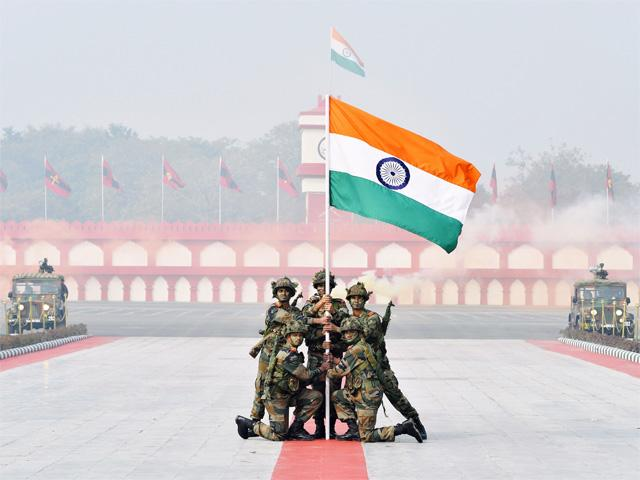
\includegraphics[height=10cm,width=10cm]{img}
\end{center}
\newpage
\tableofcontents
\newpage
\section{\textcolor{blue}{Introduction}}
In this project we will try to build a web portal for our soldier's family. The main aim of this portal is to connect common people with martyred soldier's family or disabled soldier.

Here we will provide the details of the soldier's family, their bank account numbers, and home address (if government allows). We will also provide a common bank account number where any individual can deposit any amount of money and the money will be used for the welfare of our soldier's family. 

We will also provide address based on location of the soldier's family. So that any volunteer can go there and help them. Also volunteer can celebrate festivals with their family.

\section{\textcolor{blue}{Mission}}
If a soldier martyrs while serving our nation, then it's our duty to take care of his or her parents. This project is just a small step to fulfill it.

\section{\textcolor{blue}{Advantages}}
\begin{enumerate}
  \item By this project we will be able to connect millions of soldier's family with common people.
  \item They will not feel alone in their old age.
  \item Soldier's children can fulfill their dreams.
  \item Though we will not bring back their son but we can help them as much as possible.
  \item Volunteer can also find it easy to connect with them.
\end{enumerate}

\section{\textcolor{blue}{Disadvantage}}
\begin{enumerate}
 \item The government may ban this program due to security threat.
\end{enumerate}

\section{\textcolor{blue}{Extension}}
\begin{enumerate}
 \item We can extend this project for farmers also.
\end{enumerate}
\end{document}
